\documentclass[12pt]{article}
\usepackage[utf8]{inputenc}
\usepackage[T1]{fontenc}
\usepackage[french]{babel}
\usepackage{amsmath,amsthm,amsfonts,amssymb}
\usepackage{lmodern}
\usepackage[top=2.4cm,bottom=2.4cm,left=2cm,right=2cm]{geometry}
\usepackage{hyperref}
\usepackage{multicol}
\usepackage{enumitem}
\usepackage{listings}
\usepackage[dvipsnames]{xcolor}
\usepackage{tikz}
\author{MABROUK Fayez \& AHMED-ZAID Macyl}
%\date{}
\title{{\bf Jeu de dames} \\
	Rapport de projet \\
	{\small L3 Informatique 2022-2023} \\
	{\it \small  Intelligence artificielle}}

\begin{document}
	
	
	\maketitle
		\begin{figure}[!hbtp]
		\centering
		
\includegraphics[scale=0.5]{ACTU-UPC.png}
		
	\end{figure}
	
	\newpage
	\tableofcontents
	\newpage
	\section{Introduction}
	Le jeu de dames est un jeu de société populaire et ancien qui se joue sur un plateau carré avec des cases noires et blanches. Les joueurs déplacent leurs pions diagonalement sur le plateau en essayant de capturer les pions adverses en sautant par-dessus eux. Le but du jeu est de capturer tous les pions de l'adversaire ou de le bloquer de telle sorte qu'il ne peut plus bouger. 
	\section{Démarche de programmation}
	\subsection{Diagramme de classe}
	\section{Documentation technique}
	\subsection{La classe main}
	Le code crée une fenêtre de jeu et permet à l'utilisateur de jouer contre l'IA ou de laisser l'IA jouer contre elle-même.\\
	Le code commence par définir certaines constantes telles que la taille de la fenêtre, la taille des cases de la grille, les images pour les éléments du jeu, etc. Ensuite, la fonction get row col from mouse  est définie pour déterminer la rangée et la colonne de la case sur laquelle l'utilisateur a cliqué avec la souris. Ensuite, la boucle principale du jeu est démarrée, dans laquelle la logique de jeu est mise à jour à chaque itération. La boucle gère également les événements tels que les clics de souris et la fermeture de la fenêtre.
	\subsection{La classe Board}
	 Le code définit une classe Board qui gère la logique du jeu et affiche la grille de jeu.\\
	 \\
	 Le constructeur de la classe Board initialise la grille de jeu en appelant la méthode creer grille(). La grille de jeu est stockée sous forme de liste de listes, où chaque élément est soit un objet Piece, soit la valeur 0 pour représenter une case vide. Il y a également des variables pour suivre le nombre de pions et de rois restants pour chaque joueur. \\
	 \\
	 La méthode creer cases() dessine la grille de jeu en alternant les cases bleues et blanches. La méthode ajouter pieces sur grille() dessine tous les pions et les rois sur la grille de jeu.\\
	 \\
	 La méthode change position sur grille() met à jour la position d'un pion sur la grille en échangeant sa position actuelle avec sa nouvelle position. Si un pion atteint la dernière rangée de la grille, il est promu en un roi. Les rois sont également suivis dans les variables de la classe.\\
	 \\
	 La méthode valid moves() retourne un dictionnaire de tous les mouvements valides possibles pour un pion donné. Cette méthode utilise des méthodes privées pour vérifier les mouvements diagonaux des pions, en fonction de la couleur du joueur et de l'état du pion (normal ou roi)
	 \subsection{La classe constants}
	 Cette classe définit quelques constantes de couleur et charge des images pour les couronnes et l'arrière-plan du jeu. La taille de l'écran est également définie, ainsi que le nombre de rangées et de colonnes pour le plateau de jeu.
	 \subsection{La classe Game}
	 Cette classe gère la logique du jeu de dames. Elle utilise la bibliothèque Pygame pour afficher le jeu à l'écran.\\
	 La classe "Game" a plusieurs méthodes :\\
	 La méthode "init" est appelée lorsque la classe est instanciée. Elle initialise les variables d'instance qui sont utilisées pour suivre l'état du jeu.\\
	 \\
	 La méthode "update" met à jour l'affichage du jeu à l'écran. Elle appelle la méthode "ajouter pieces sur grille" de l'objet "board" pour dessiner les pièces sur la grille de jeu. Elle appelle également la méthode "afficher valid moves" pour dessiner les mouvements valides.\\
	 \\
	 La méthode "init" initialise les variables d'instance de la classe.\\
	 \\
	 La méthode "reset" réinitialise les variables d'instance pour commencer une nouvelle partie.\\
	 \\
	 La méthode "winner" retourne le gagnant de la partie.\\
	 \\
	 La méthode "choisir piece" est appelée lorsque le joueur choisit une pièce. Elle vérifie si la pièce sélectionnée appartient au joueur actuel, et si c'est le cas, elle stocke cette pièce dans la variable "selected" et calcule les mouvements valides pour cette pièce.\\
	 \\
	 La méthode " is piece choisie" vérifie si une pièce a été sélectionnée.\\
	 \\
	 La méthode " is moved" est appelée lorsque le joueur déplace une pièce. Elle vérifie si la case de destination est valide et déplace la pièce sélectionnée. Si une pièce a été sautée, elle est supprimée de la grille.\\
	 \\
	 La méthode "changer tour" change le tour du joueur.\\
	 \\
	 La méthode "afficher valid moves" dessine des cercles verts sur les cases de destination valides pour la pièce sélectionnée.\\
	 \\
	 La méthode "ai move" est appelée lorsqu'un mouvement est effectué par l'IA. Elle met à jour l'état de la grille.\\
	 \\
	 La méthode "get board" retourne l'objet "board" de la classe "Game".
	 \subsection{La classe algorithm}
	 Cette classe contient une fonction minimax qui utilise l'algorithme de minimax pour trouver le meilleur coup pour un joueur donné. La fonction prend en entrée la position actuelle, la profondeur de recherche et un booléen max player indiquant si le joueur est le joueur maximisant ou minimisant. La fonction renvoie une paire (valeur, coup) où la valeur est la valeur d'utilité de la position et le coup est le meilleur coup trouvé.\\
	 \\
	 La fonction utilise une fonction auxiliaire get all moves pour générer tous les coups possibles pour un joueur donné. La fonction simulate move est également utilisée pour simuler un coup sur une copie temporaire du plateau de jeu.
	 \subsection{La classe Piece}
	 Cette classe représente une pièce de jeu de dames sur le plateau. Elle possède des attributs tels que row, col, color et king (si la pièce est devenue une dame ou non). Elle possède également des méthodes telles que calc pos (qui calcule la position de la pièce sur le plateau), get king (qui définit l'attribut king à True), create piece (qui dessine la pièce sur le plateau en utilisant la bibliothèque Pygame) et move piece (qui met à jour la ligne et la colonne de la pièce et recalcule sa position).
	 \section{Guide d'utilisation}
	 	%\begin{figure}[!hbtp]
%	 	\centering
%	 	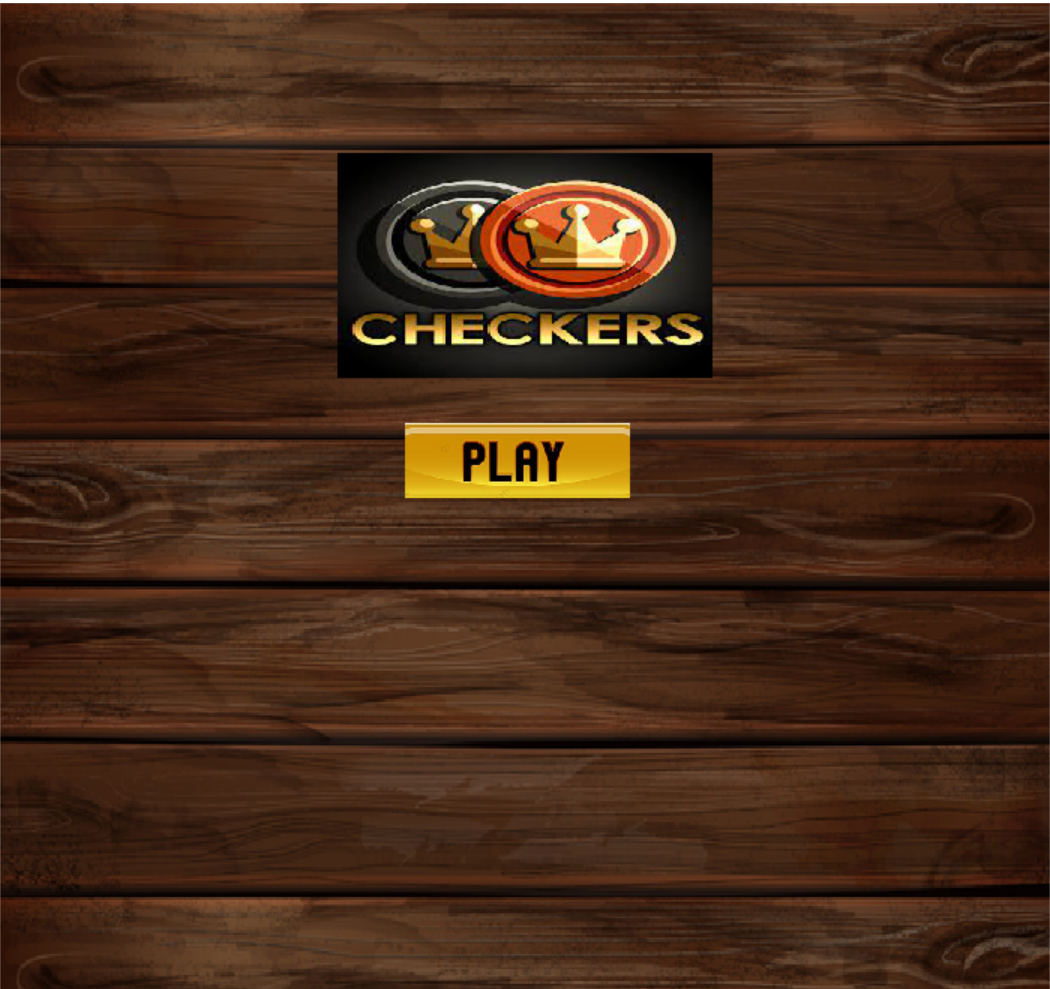
\includegraphics[scale=0.5]{Capture.png}
	 	
%	 \end{figure}
 %	\begin{figure}[!hbtp]
 %	\centering
 %	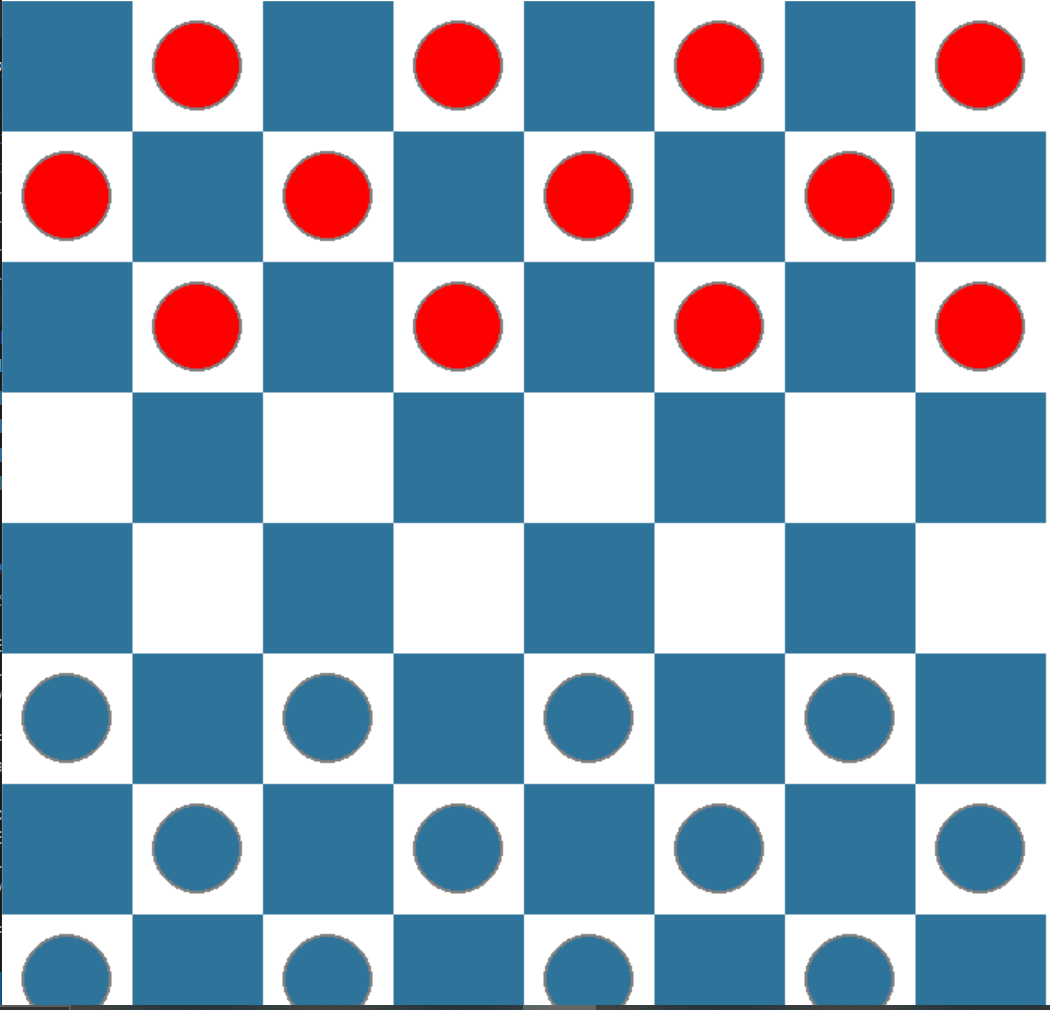
\includegraphics[scale=0.5]{Capture1.png}
 	
 %\end{figure}
 \begin{figure}[h]
 	\centering
 	\begin{minipage}[b]{0.45\linewidth}
 		\centering
 		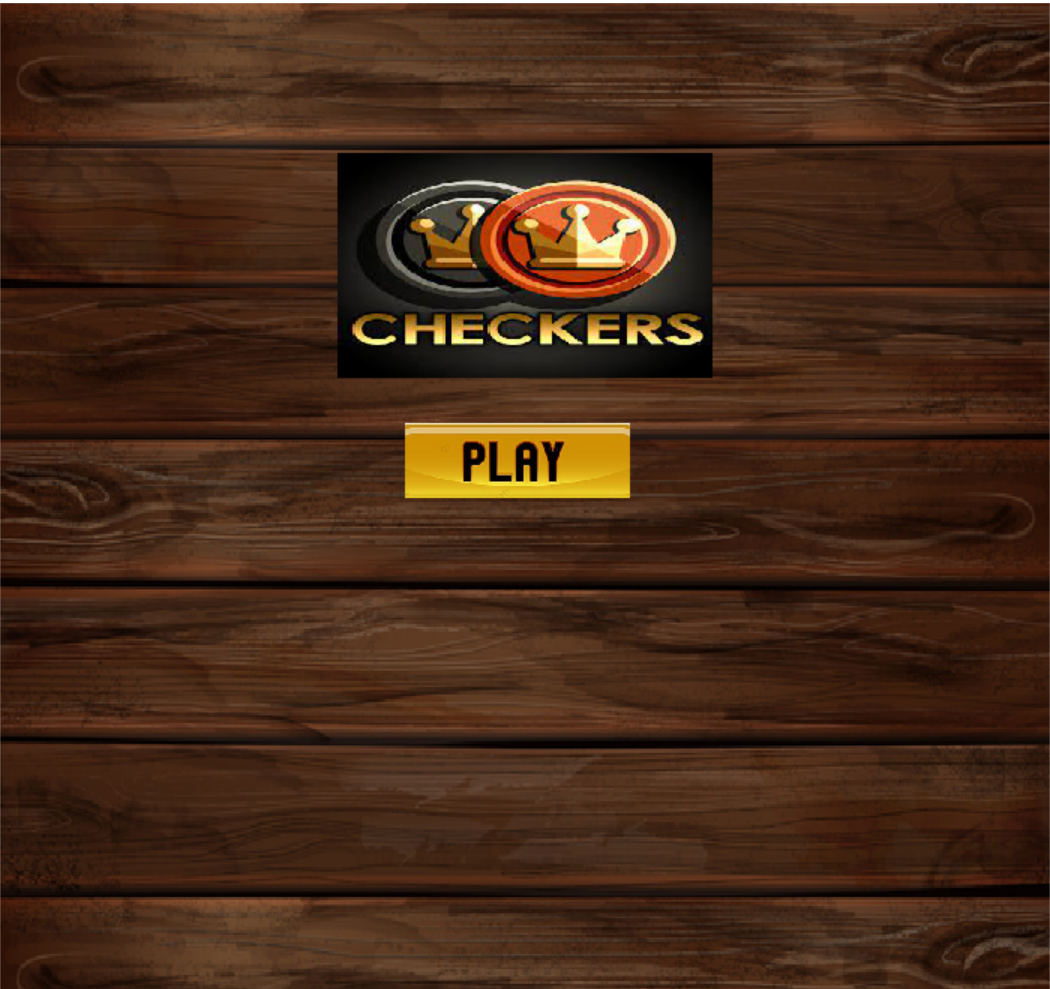
\includegraphics[width=\textwidth]{Capture.png}
 		\caption{Menu de jeu}
 	\end{minipage}
 	\hfill
 	\begin{minipage}[b]{0.45\linewidth}
 		\centering
 		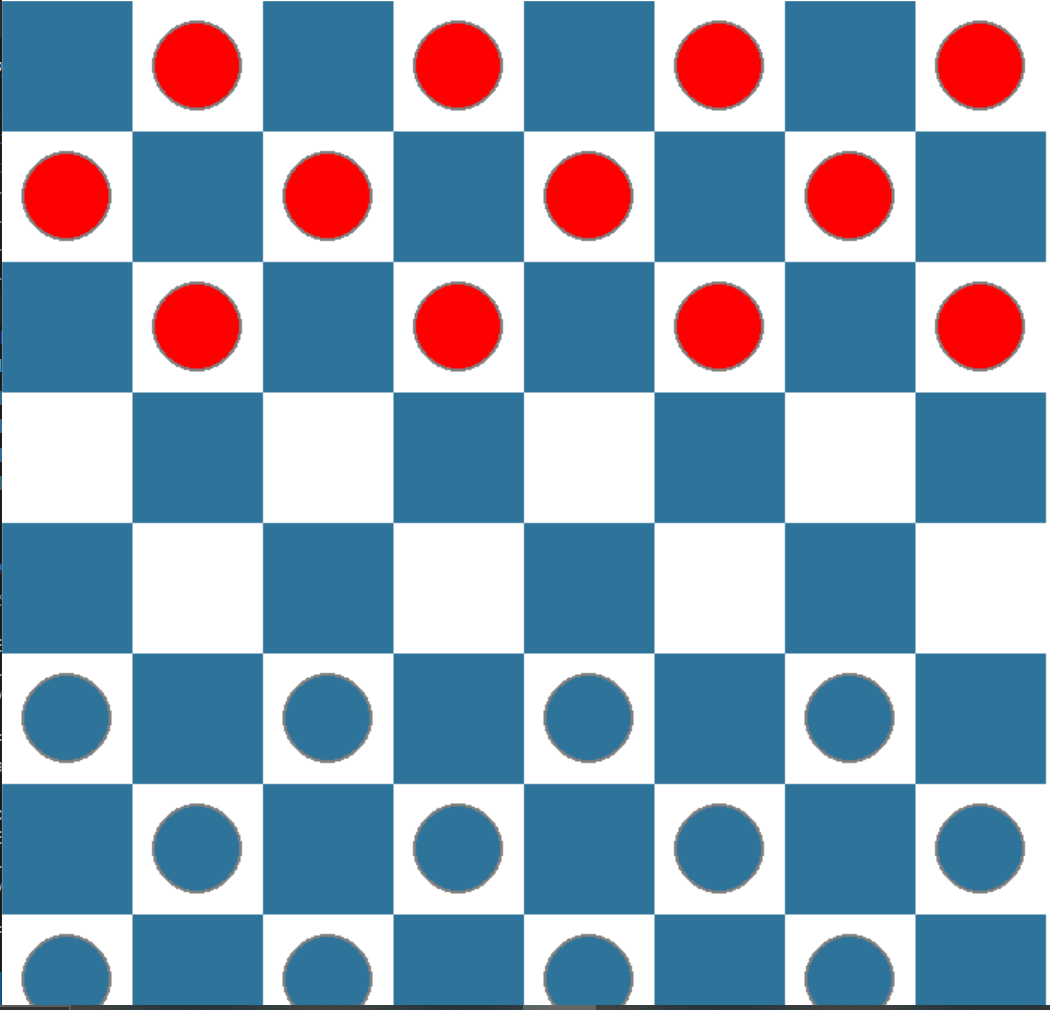
\includegraphics[width=\textwidth]{Capture1.png}
 		\caption{Plateau de jeu}
 	\end{minipage}
 \end{figure}
	\section{Conclusion}
	Ce projet de jeu de dames a été une excellente occasion d'apprendre à programmer des jeux en utilisant Python et la bibliothèque Pygame. Le jeu a été développé en plusieurs étapes, en commençant par la création de la grille de jeu et la mise en place des pièces de jeu. Ensuite, les mouvements des pièces ont été implémentés, suivis de la sélection des pièces et de la mise en évidence des mouvements valides possibles.\\
	
	L'implémentation de l'IA utilisant l'algorithme minimax a permis d'ajouter une nouvelle dimension passionnante au jeu. L'IA est capable de prévoir les coups à venir et de choisir la meilleure option en fonction de sa profondeur de recherche.\\
	
	En résumé, ce projet a été un excellent moyen de mettre en pratique les compétences de programmation en Python, en utilisant la bibliothèque Pygame pour créer un jeu de dames entièrement fonctionnel, et en ajoutant une IA pour permettre de jouer contre l'ordinateur. Il a également fourni une occasion de réfléchir à des algorithmes d'IA tels que minimax, qui peuvent être appliqués à d'autres jeux et problèmes.
\end{document}